%
% Complete documentation on the extended LaTeX markup used for Insight
% documentation is available in ``Documenting Insight'', which is part
% of the standard documentation for Insight.  It may be found online
% at:
%
%     http://www.itk.org/

\documentclass{InsightArticle}


%%%%%%%%%%%%%%%%%%%%%%%%%%%%%%%%%%%%%%%%%%%%%%%%%%%%%%%%%%%%%%%%%%
%
%  hyperref should be the last package to be loaded.
%
%%%%%%%%%%%%%%%%%%%%%%%%%%%%%%%%%%%%%%%%%%%%%%%%%%%%%%%%%%%%%%%%%%
\usepackage[dvips,
bookmarks,
bookmarksopen,
backref,
colorlinks,linkcolor={blue},citecolor={blue},urlcolor={blue},
]{hyperref}
% to be able to use options in graphics
\usepackage{graphicx}
% for pseudo code
\usepackage{listings}
% subfigures
\usepackage{subfigure}


%  This is a template for Papers to the Insight Journal. 
%  It is comparable to a technical report format.

% The title should be descriptive enough for people to be able to find
% the relevant document. 
\title{Efficient implementation of kernel filtering}

% Increment the release number whenever significant changes are made.
% The author and/or editor can define 'significant' however they like.
% \release{0.00}

% At minimum, give your name and an email address.  You can include a
% snail-mail address if you like.
\author{Richard Beare{$^1$} {\small{and}} Ga\"etan Lehmann{$^2$}}
\authoraddress{{$^1$}Department of Medicine, Monash University, Australia.\\
{$^2$}INRA, UMR 1198; ENVA; CNRS, FRE 2857, Biologie du D\'eveloppement et
Reproduction, Jouy en Josas, F-78350, France}

\begin{document}
\maketitle

\ifhtml
\chapter*{Front Matter\label{front}}
\fi


\begin{abstract}
\noindent
% The abstract should be a paragraph or two long, and describe the
% scope of the document.
Kernel based filtering is one of the fundamental tools of image
analysis and processing. A number of approaches have been developed
over the years that allow efficient implementation of such filters
even when the kernel size is large. This article reviews some of these
methods and introduces their ITK implementations.
\end{abstract}

\tableofcontents

\section{Introduction}
A kernel based filtering process replaces the pixel at the kernel
origin with the result of a function of all pixels defined by
the kernel. Many useful filters, including edge detection and gradient
filters, smoothing filters and rank and morphology filters fall into
this category. Direct implementations of such filters typically
involve visiting all pixels defined by the kernel in order to evaluate
the filter function. Such an approach is usually easy to implement
-- in ITK it is made simple by the neighborhood iterators -- but leads
to an algorithm complexity proportional to the number of pixels in the
kernel (or $O(n^d)$, where $n$ is the kernel size and $d$ is the
dimensionality). Such complexity tends to restrict application of such
filters to small kernels.

A number of classical methods exist for reducing this complexity to
more manageable, in some cases kernel size independent, levels. ITK
already exploits such techniques for Gaussian convolution
operations. This paper describes the classical techniques for
optimized mathematical morphology filters, rank filters and certain
convolution filters. These filters make the use of large kernels,
which can be very useful in many applications, practical on
conventional computing hardware.

\section{Separability and recursive implementations}
The two approaches most typically used to reduce complexity of kernel
based filters are separability and recursive computation, both of
which are used in the ITK implementation of Gaussian convolution
filters. A separable filter implements a multidimensional kernel by
cascading several one dimensional kernels, therefore reducing
complexity from $O(n^d)$ to $O(nd)$. The second approach exploits
redundancy that might be present in the computations of kernel
functions at neighboring locations, leading, in some cases, to a complexity
independent of $n$.

\section{Mathematical morphology operations}
Two optimized forms of the mathematical morphology operations of
erosion, dilation, opening and closing are presented here. The kernel
is usually referred to as the structuring element in mathematical
morphology. The methods described here are applied to ``flat''
structuring elements, that is structuring elements without
weights. The first method can be applied to arbitrary structuring
elements while the second can be applied to line structuring elements.

\subsection{Arbitrary structuring elements}
\label{sect:MMmovingHist}
The method described in \cite{Vandroogenbroeck96.3} relies on the
simple concept of an up-datable histogram, and is often described as a
``moving histogram'' approach. A histogram is computed for a kernel
located at the first voxel. The histogram at the neighboring voxel can
then be computed by including newly included voxels and removing newly
excluded voxels. The list of included and excluded voxels
corresponding to movement in any direction can be computed when the
structuring element is created, and the direction with the smallest
number of changes should be selected as the direction for sweeping the
kernel across the image. The erosion or dilation at each location is
computed by selecting the minimum or maximum from the histogram. This
approach is very efficient when 8 or 16 bit pixels are used because
the histogram can be represented as an array and the histogram updated
by incrementing or decrementing the appropriate bins. Using place
holders to track the current maximum or minimum increases
performance. More sophisticated histogram representations are
necessary for larger pixel types. Our implementation uses c++ maps,
which is an extension to the original paper.

This methodology reduces the complexity from $O(n^d)$ to $O(n^{d-1})$,
while keeping the structuring element identical to the direct
implementation.

\subsection{Decomposition of structuring elements}
\label{sect:MMdecomp}
Morphological erosions and dilations are separable -- successive
dilation by orthogonal lines is equivalent to dilation by a rectangle
with sides equal to the line lengths. This means that any
hyper-rectangular structuring element can be constructed using several
orthogonal lines, typically parallel to the axes.

Approximations of more complex shapes, notably circles and
ellipses can constructed using a number of lines at evenly spaced
angles \cite{Adams93}. It is difficult to create a structuring element
with a precisely defined radius using this method because line
structuring elements from which the circle structuring element is
composed must have odd length and there are practical limits due to
the realities of underlying digital grid representation of images. In
addition it is possible that the structuring elements may not be truly
translation invariant due to the representation of line
(e.g. Bresenham) used in the decomposition. However, precisely defined
radii are rarely critical when a large structuring element is called
for. An example of a structuring element created using line
structuring elements is shown in Figure
\ref{fig:circledecomposition}. Composition of regular shapes, such as
hexagons and octagons is more accurate.

\begin{figure}[htbp]
\centering

\includegraphics{kernel}
\caption{Approximate circular structuring element, radius 25, constructed using 8 lines.\label{fig:circledecomposition}}
\end{figure}

It is also possible, in theory, to construct 3D structuring elements
in similar ways. The construction of a hyper-rectangle is trivial,
however construction of spheres is more problematic. The code
discussed later provides preliminary implementations based on some
platonic solids and various spherical approximations, but further
testing and development is needed.

\subsection{Line structuring elements}
The decompositions discussed above are important because an efficient,
recursive, implementation of erosion and dilations along lines
exists. This method was introduced in \cite{Gil1993,vanHerk1992a} and
can compute an erosion or dilation in 3 operations per pixel,
independent of structuring element length. \cite{Gil2000} recently
reduced the cost to 1.5 pixels per pixel, but the procedure is more
complicated and there are reports of no speedup in practice.

The original algorithms utilize forward and backward running maxima
(for dilation) for the length of the structuring element from a pixel
of interest. The dilation can then be computed for a region the size
of the structuring element around the point of interest by comparing
values on the running extrema that are separated by the structuring
element length. This is illustrated in Figure \ref{fig:vHGWmethod}

\begin{figure}[htbp]
\centering
\includegraphics[scale=0.5]{vHGWexpl}
\caption{The van Herk, Gil, Werman method.\label{fig:vHGWmethod}}
\end{figure}

A method known as {\em anchor morphology} has been published recently
\cite{Vandroogenbroeck2005Morphological} that offers improved
performance and the ability to perform a line opening directly (rather
than using an erosion/dilation cascade). This method has been
implemented in the filters discussed later in the article, but
performance issues are not yet clear. The method employs histograms
and therefore needs more complex data structures when applied to
higher precision data, potentially reducing any speed advantage.

\begin{figure}[htbp]
\begin{center}
\subfigure[Input]{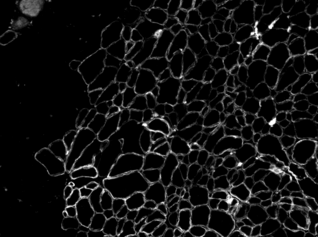
\includegraphics[scale=1.88]{CellsFluorescence2}}
\subfigure[Dilation]{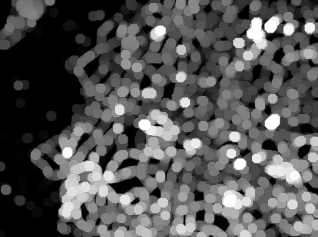
\includegraphics[scale=0.45]{dilate2D-std}}
\subfigure[Erosion]{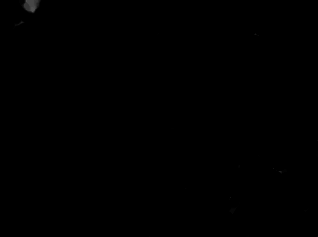
\includegraphics[scale=0.45]{erode2D-std}}
\subfigure[Opening]{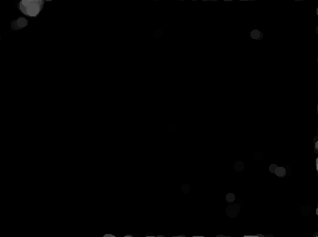
\includegraphics[scale=0.45]{open2D-std}}
\subfigure[Closing]{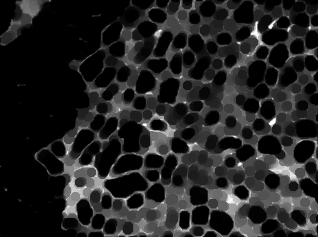
\includegraphics[scale=0.45]{close2D-std}}
\subfigure[White top-hat]{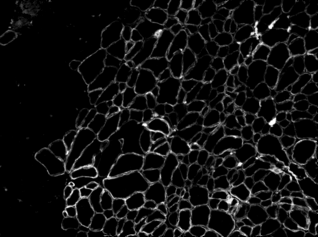
\includegraphics[scale=0.45]{whiteTopHat2D-std}}
% \subfigure[Gradient]{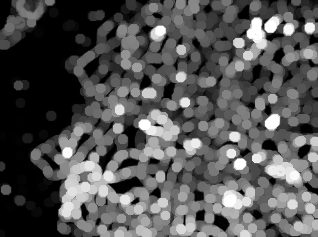
\includegraphics[scale=0.5]{gradient2D-std}}
\caption{Effect of a dilation (b), an erosion (c), an opening (d),
a closing (e) and a white top hat (f) with a ball structuring element.}
\end{center}
\end{figure}


\section{Rank filters}
\label{sect:rank}
Efficient implementations of median and rank filters can be carried out
using exactly the same approach as discussed for morphological
operations with arbitrary structuring elements. The method was
originally proposed in \cite{Huang79}. The implementation discussed
later supports arbitrary kernel shapes and pixel types as well as any
choice of rank.

Rank filters are not separable. However the performance benefits
offered by separability make it worth pretending they are. If median
filtering is being used to provide robust noise filtering or
background estimation then a separable approximation is worth
testing. This concept was originally proposed in \cite{Narendra81}. In
fact it is also possible to apply the decomposition discussed in
Section \ref{sect:MMdecomp} to median filters to achieve a closer
approximation to circular kernels.

\section{Mean and standard deviation filters}
\label{sect:meanVar}
A simplified version of the moving histogram approach can also be used
to efficiently compute the mean or standard deviation of an arbitrarily shaped
kernel. The histogram used for morphology and rank filters is a data
structure that, once established for one pixel, can be easily updated
to represent the kernel for a neighboring pixel. The data structure
required to perform the equivalent function for mean and variance
operations is much simpler -- all that is necessary is the sum of
pixel values under the kernel (or sum of squared values for variance
calculations), and the kernel size. The sum can be updated by adding
the new values and subtracting the old and the output computed by
dividing by the kernel size.

A more efficient strategy was proposed in \cite{Crow84} for
rectangular kernels. This approach first computes an accumulator image
in which each $i,j$ is replaced by the sum of voxels ``left'' and
``above'' it. This accumulator image may be computed recursively using
local neighborhood values. The mean of rectangles of any size may then
be computed using accumulated values at the rectangle corners. Figures
\ref{fig:accum} and \ref{fig:accumMean} illustrate the 2D case and the
update formulas are provided in Equations \ref{eq:accum}, \ref{eq:accSum}, and
\ref{eq:accumMean}.

\begin{eqnarray}
\label{eq:accum}
b_{i,j} & = & \sum_{x \leq i, y \leq j} a_{x,y} \\ \nonumber
	& = & b_{i,j-1} + b_{i-1, j} + a_{i,j} - b_{i-1, j-1}
\end{eqnarray}
where $b_{i,j}$ is the accumulator value at location $i,j$ and $a_{i,j}$ is the input image intensity at $i,j$.

\begin{equation}
\label{eq:accSum}
S_{i,j} = b_{i+w/2,j+h/2} + b_{i-w/2,j-h/2} - b_{i-w/2,j+h/2} + b_{i+w/2,j-h/2}
\end{equation}
where $S_{i,j}$ is the sum of the pixel values in the neighborhood centered at $i,j$.

\begin{equation}
\label{eq:accumMean}
m_{i,j} = \frac{1}{w.h}S_{i,j}
\end{equation}
where $m_{i,j}$ is the output of the mean filter at location $i,j$.

Using the same strategy, the standard deviation can be efficiently
computed.  It requires an accumulator image of the squared pixels
values, which can be efficiently computed at the same time as the
original accumulator image. The update formulas are provided in
Equations \ref{eq:accum2}, \ref{eq:accSum2} and \ref{eq:accumSigma}.

\begin{eqnarray}
\label{eq:accum2}
b2_{i,j} & = & \sum_{x \leq i, y \leq j} a_{x,y}^2 \\ \nonumber
	& = & b2_{i,j-1} + b2_{i-1, j} + a_{i,j}^2 - b2_{i-1, j-1}
\end{eqnarray}
where $b2_{i,j}$ is the accumulator value at location $i,j$ for the square image, and $a_{i,j}$ is the input image intensity at $i,j$.

\begin{equation}
\label{eq:accSum2}
S2_{i,j} = b2_{i+w/2,j+h/2} + b2_{i-w/2,j-h/2} - b2_{i-w/2,j+h/2} + b2_{i+w/2,j-h/2}
\end{equation}
where $S2_{i,j}$ is the sum of the squared pixel values in the neighborhood centered at $i,j$.

\begin{equation}
\label{eq:accumSigma}
\sigma_{i,j} = \sqrt{\frac{S2_{i,j} - \frac{S_{i,j}^2}{w.h}}{w.h-1}}
\end{equation}
where $\sigma_{i,j}$ is the output of the standard deviation filter at location $i,j$.

\begin{figure}[htbp]
\centering
\includegraphics[scale=0.5]{accum2D}
\caption{Recursive computation of the accumulator image - value at $(i,j)$ computed using Equation \ref{eq:accum}. The double hashed region is subtracted because it is included in both $b_{i,j-1}$ and $b_{i-1, j}$.\label{fig:accum}}
\end{figure}

\begin{figure}[htbp]
\centering
\includegraphics[scale=0.5]{accumMean2d}
\caption{Computation of mean using the accumulated image - value at $(i,j)$ computed using Equation \ref{eq:accumMean}.\label{fig:accumMean}}
\end{figure}

This approach to convolution has been used recently in face detection
applications \cite{Viola2004}, where rectangular filters of many
different sizes and shapes were needed and could be computed from the same accumulation image.

\begin{figure}[htbp]
\begin{center}
\subfigure[Input]{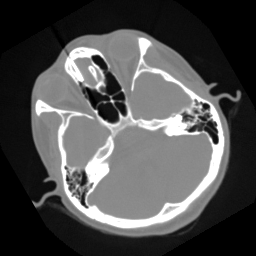
\includegraphics[scale=0.6]{cthead1}}
\subfigure[Mean]{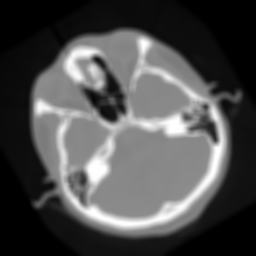
\includegraphics[scale=0.6]{test}}
\subfigure[Sigma]{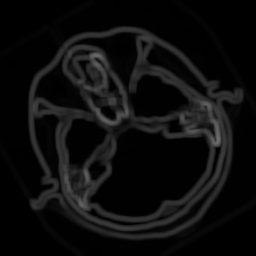
\includegraphics[scale=0.6]{sigma}}
\caption{A mean transform (b) and a standard deviation transform (c) with a kernel of radius 3.}
\end{center}
\end{figure}


\section{ITK implementation}
The filters discusses in this article are contained in 3 packages --
{\em consolidatedMorphology}\footnote{An earlier version of the {\em consolidatedMorphology} package has
been submitted to the InsightJournal. However many improvements and
bug fixes have been included since then.}, {\em fastRankMean} and {\em
boxConvolution}. The most recent versions of these packages can be
obtained from \url{http://voxel.jouy.inra.fr/darcsweb/}\footnote{
The most recent versions can be obtained using darcs \cite{DarcsWebSite}
with the command {\em darcs get http://voxel.jouy.inra.fr/\\darcs/contrib-itk/package},
where {\em package} must be replace by {\em consolidatedMorphology},
{\em fastRankMean} or {\em boxConvolution}.}.
All of the packages
include multithreaded filters and include many examples and tests. Unless
indicated otherwise, all filters will behave basically the same way as
other kernel filters, requiring either a radius or a neighborhood to
be specified.

\subsection{Morphology filters -- consolidatedMorphology}


The morphology filters utilize a new class -- {\em
FlatStructuringElement} to describe, arbitary and decomposable
structuring elements. It provides the following methods to create
structuring elements with different characteristics:
\begin{itemize}
  \item \verb$Ball()$ generate a ball structuring element (a circle in 2D). It takes the 
	radius of the structuring element as parameter.
  \item \verb$Box()$ produces a box structuring element. It takes the radius 
	of the structuring element as parameter.
  \item \verb$Poly()$ produces an approximation to a circle or sphere using 
	line structuring elements, taking the desired radius and number of 
	lines as parameters. In the 3D case an approximation of a sphere will 
	be attempted. Caution is advised because this is not well tested yet.
  \item \verb$FromImage()$ produces a structuring element from an image. The image is passed
as parameter to the method. A optional parameter can also be passed: the pixel value
to be considered as the foreground value in the image. This value defaults to
\verb$NumericTraits< PixelType >::max()$. This lets the user visualize the structuring element.
\end{itemize}

The algorithm used by a filter is set by the {\em SetAlgorithm}
method, with options of {\em BASIC}, {\em HISTO}, {\em VHGW} and {\em
ANCHOR}, for the traditional ITK implementation, the moving histogram
algorithm, the van Herk, Gil, Werman algorithm and the anchor
algorithm respectively. The VHGW and ANCHOR algorithms can only be
used for Box and Poly structuring elements. VHGW is more thoroughly
tested. The HISTO algorithm produces the identical results to BASIC,
and is always faster. It is the default and should be used if you need
precisely defined, non rectangular, structuring elements. If a Box
structuring element is needed then VHGW or ANCHOR should be used, as
they offer the best performance and are exact in that case. Poly
structuring elements are approximations of circles that will offer
improved performance with VHGW or ANCHOR algorithms, but the user will
need to consider whether the approximation is suitable for the
application in question.

The availability of line morphology operations means that new
operations, such as ``union of openings'' can be implemented easily.

\subsection{Rank and mean filters -- fastRankMean}
The {\em fastRankMean} packge uses the sliding window method to
implement rank and mean filters for arbitary kernel shapes. It also
uses line versions of these kernels to provide a ``separable rank''
filter -- an fast approximation to a real rank filter as discussed in
Section \ref{sect:rank}. There are also a number of filters that
accept a mask input and return the rank or mean value of the
intersection of kernel and mask. These are experimental and haven't
been thoroughly tested. The filters are {\em itkRankImageFilter,
itkMovingWindowMeanImageFilter, itkFastApproxRankImageFilter,
itkFastApproxMaskRankImageFilter} and {\em
itkMaskedRankImageFilter}. itkRankImageFilter implements arbitary
shaped kernels, itkFastApproxRankImageFilter implements the separable
approximation and itkMovingWindowMeanImageFilter implements an
arbitary shaped kernel mean.

\subsection{Rectangular convolution -- boxConvolution}
The {\em boxConvolution} uses the accumulation method described in
Section \ref{sect:meanVar} to implement rectangular mean and variance
computations. The filters implement different boundary conditions to
{\em itkMeanImageFilter}, with the mean of the kernel inside the image
being computed. The filters in this package are multithreaded and deal
with arbitrary dimensions. The current filters do not support the mode
of operation used in face recognition application in which an
accumulation image is repeatedly ``queried'' for mean values of
various sized kernels. However introducing such a capability is
relatively easy.

\subsection{Extended languages support}

All the new filters provided are wrapped using WrapITK's external projects
\cite{WrapITK} and have been successfully tested with python.

\section{Performance}

All the execution times in this section are measured on a computer with four
Intel\textregistered Xeon\textregistered CPU cores at 2.33GHz with 4MB cache,
running CentOS 4.4 64 bits. Unless specified in the description, the tests are
forced to run on a single core.

\subsection{Morpholgy}

Execution times for the dilation, the opening, and the gradient transform are shown in
Tables \ref{tab:perfDilation}, \ref{tab:perfOpening} and \ref{tab:perfGradient}, and in
Figure \ref{fig:consolidatedMorphology-perf}. The predicted linear complexity for the number
of neighbors is observed for the basic algorithm, as well as the constant complexity of the
van Herk / Gil Werman and the anchor algorithm. The linear complexity for the number of
pixels added and removed per translation is observed for the moving histogram algorithm,
as expected.

A good threading support is observed for all the implementations, as shown in Table
\ref{tab:perfThreads} and Figure \ref{fig:consolidatedMorphology-perf}.

\begin{figure}[htbp]
\begin{center}
\subfigure[Dilation]{\includegraphics[scale=0.62]{consolidatedMorphology-perf2D-dilation-small}}
\subfigure[Opening]{\includegraphics[scale=0.62]{consolidatedMorphology-perf2D-opening-small}}
\subfigure[Gradient]{\includegraphics[scale=0.62]{consolidatedMorphology-perf2D-gradient-small}}
\subfigure[Threads]{\includegraphics[scale=0.62]{consolidatedMorphology-perf_threads}}
\subfigure[Number of neighbors]{\includegraphics[scale=0.62]{consolidatedMorphology-perf_nb_of_neighbors}}
\subfigure[Polygon]{\includegraphics[scale=0.62]{consolidatedMorphology-perf2Dpoly}}
\caption{Execution times with a box structuring element of increasing size for different algorithms of dilation (a),
opening (b) and gradient (c).
Execution times with and increasing number fo threads (d).
Execution times with an increasing number of neighbors in a box structuring of constant radius (e).
Execution times with a polygon structuring element. The polygon approximations use the default number of lines (a maximum of 6 when radius is greater than 8 (f).\label{fig:consolidatedMorphology-perf}
Results are reported in Tables \ref{tab:perfDilation}, \ref{tab:perfOpening}, \ref{tab:perfGradient},
\ref{tab:perfThreads} and \ref{tab:perf2Dpoly}.
}
\end{center}
\end{figure}

\subsection{Rank and Mean filters}
Relative times for sliding window median and mean filters and
separable median filters are shown in Tables \ref{tab:perfRankMean}
and \ref{tab:perfRankMedian} and in Figure \ref{fig:perfRank}. The
predicted linear complexity is observed for the sliding window
approaches (complexity of direct approach is $O(n^2)$ in 2D, reduced
to $O(n)$ by using the sliding window. The separable median exhibits a
runtime independent of kernel size, as expected.

\begin{figure}[htbp]
\begin{center}
\subfigure[Mean]{\includegraphics[scale=0.62]{fastRankMean-perfMean}}
\subfigure[Median]{\includegraphics[scale=0.62]{fastRankMean-perfMedian}}
\caption{Execution times for several algorithms of mean filters (a) and
median filters (b).\label{fig:perfRank}
Results are reported in Tables \ref{tab:perfRankMean} and  \ref{tab:perfRankMedian}.}
\end{center}
\end{figure}


\subsection{Box Convolution}
The relative times for optimized and standard convolution are shown in
Table \ref{tab:perfBoxConv} and Figure \ref{fig:perfBoxConv}, and demonstrate significantly improved
performance for kernel radii greater than 1. The times support the
theoretical prediction that the complexity of the algorithm is
independent of kernel size.

A good threading support is observed for all the implementations, as shown in Table
\ref{tab:perfBoxConv-threads} and Figure \ref{fig:perfBoxConv}.


\begin{figure}[htbp]
\begin{center}
\subfigure[Neighborhood size]{\includegraphics[scale=0.62]{boxConvolution-perf2D-large}}
\subfigure[Threads]{\includegraphics[scale=0.62]{boxConvolution-perf_threads-large}}
\caption{Execution times for and increasing kernel size (a), and an increasing number of threads (b).
\label{fig:perfBoxConv}
Results are reported in Tables \ref{tab:perfBoxConv} and  \ref{tab:perfBoxConv-threads}}
\end{center}
\end{figure}




\subsection{Timing notes}
You may have noticed that the optimized filters of radius 1 seem to
regularly perform slower than their larger counterparts. We can think
of no reason for this. The algorithms that have kernel size
independent complexity should not be slower for small kernels than
large ones because the only difference occurs at borders and when the
sliding window is being created, and both situations favour small
kernels. We can only guess that there are caching issues involved.

\section{Implementation Notes}
A lot of effort has been spent implementing and optimizing these filters 
while attempting to maintain good ITK style. This section summarizes some observations
and experiences:
\subsection{Moving histograms}
The most obvious way of implementing moving histograms involves
neighborhood iterators.  However the resulting performance wasn't good
-- it appears that neighborhood iterator complexity is proportional to
radius rather than the number of active neighbors. A method using
lists of offsets combined with image Get/SetPixel methods approach was
used instead.

The original paper recommended moving the window in a zig-zag pattern, i.e horizontally 
across a the first row, down a step to the second row and then back, but this involves
accessing data in a reverse raster order which can potentially reduce cache performance.
An alternative has been implemented that always moves the window in forward raster direction,
at the cost of additional histogram copies, has been implemented and exhibits improved
performance for large images. Differences for small images weren't detectable.

\subsection{16 bit data types}
Histograms for 16 bit data types can be implemented using arrays or maps. One would
expect arrays to offer a simpler and therefore faster implementation, but our results
have been mixed. Presumably the performance depends significantly on voxel statistics.

\subsection{Line Operations}
The van Herk/Gil and Werman and anchor methods operate on image transects, potentially
at any angle. The transect data needs to be extracted from the image and the processed
transect written back, with successive parallel transects being processed. 
Existing iterators don't do this particularly efficiently, so image Get/SetPixel operations 
are being used. This approach isn't ideal either and needs to be worked on. In general
there is no need for boundary checks because the intersection between transect and image region
is calculated, so a potentially random access method without boundary checks would be ideal.

Building dimension independent code also adds complexity to this filter which can be avoided in
dimension specific implementations. The process of sweeping the transect across the image region
is much more complex (and therefore slower) when written in a dimension independent fashion.

The standard ITK threading approach isn't ideal for this style of filtering either -- a better 
option would be splitting the image based on transects instead of blocks. Obviously this
sort of change isn't practical.

\subsection{Refactoring}
The three packages do share some components, and some refactoring is
called for. This most widely used components are histograms and
sliding window infrastructure, which need to be consolidated.

All the kernel based filters in ITK would also benefit to hinerit a common
super class which manage the neighborhood size and/or the kernel, and which
provide the infrastructure for the separable operations.

\section{Comments and Conclusions}
This article has provided background theory for and implementations of
a number of important approaches to kernel based filtering. These
methods significantly reduce complexity and execution time, by some
orders of magnitude in many cases. These approaches are all well
established in the literature but weren't available in
ITK. Availability of filtering algorithms which are always fast,
irrespective of the kernel size, can make much simpler approaches to
many problems practical.

\section{Acknowledgments}
We thank Dr Pierre Adenot and MIMA2 confocal facilities
(\url{http://mima2.jouy.inra.fr}) for providing the 3D test image.
We are grateful to the INRA MIGALE bioinformatics platform
(\url{http://migale.jouy.inra.fr}) for providing the computational resources
used for the timing tests.

\appendix

\begin{table}[phtb]
\centering
\begin{tabular}{ccccccc}
\hline
Radius	&	Basic	&	Separable	&	Histogram	&	Separable histogram	&	Anchor	&	van Herk / Gil Werman	\\
\hline
1	&	0.00477	&	0.00491	&	0.013	&	0.012	&	0.0144	&	0.00725	\\
2	&	0.0114	&	0.0101	&	0.0161	&	0.0119	&	0.0135	&	0.00743	\\
3	&	0.024	&	0.0146	&	0.0193	&	0.0116	&	0.0129	&	0.00794	\\
4	&	0.0444	&	0.0192	&	0.0231	&	0.0114	&	0.0126	&	0.00755	\\
5	&	0.0714	&	0.0247	&	0.0261	&	0.0114	&	0.0121	&	0.0074	\\
6	&	0.107	&	0.0299	&	0.0313	&	0.0116	&	0.0127	&	0.00771	\\
7	&	0.153	&	0.034	&	0.0358	&	0.0113	&	0.0121	&	0.00859	\\
8	&	0.211	&	0.0407	&	0.038	&	0.0112	&	0.0121	&	0.00773	\\
9	&	0.281	&	0.0442	&	0.0434	&	0.0114	&	0.012	&	0.00779	\\
10	&	0.365	&	0.0486	&	0.0446	&	0.0111	&	0.0118	&	0.00763	\\
15	&	1.03	&	0.074	&	0.0604	&	0.0115	&	0.0116	&	0.00794	\\
20	&	2.23	&	0.104	&	0.079	&	0.0113	&	0.0113	&	0.00762	\\
25	&	4.11	&	0.129	&	0.0968	&	0.0114	&	0.0116	&	0.0079	\\
30	&	6.82	&	0.154	&	0.111	&	0.0114	&	0.0115	&	0.00781	\\
40	&	15.4	&	0.214	&	0.153	&	0.0116	&	0.0116	&	0.00785	\\
50	&	29.3	&	0.285	&	0.19	&	0.0119	&	0.0117	&	0.00804	\\
100	&	226	&	0.767	&	0.355	&	0.0129	&	0.0117	&	0.00809	\\
\hline
\hline
\end{tabular}
\caption{Execution times in seconds for dilation by boxes using several algorithm implementations applied to the $256 \times 256$ cthead image.\label{tab:perfDilation}}
\end{table}


\begin{table}[phtb]
\centering
\begin{tabular}{ccccc}
\hline
Radius	&	Basic	&	Histogram	&	Anchor	&	van Herk / Gil Werman	\\
\hline
1	&	0.0107	&	0.0124	&	0.0219	&	0.014	\\
2	&	0.0235	&	0.0167	&	0.0201	&	0.0144	\\
3	&	0.0488	&	0.0211	&	0.019	&	0.0154	\\
4	&	0.0895	&	0.0247	&	0.0184	&	0.0148	\\
5	&	0.143	&	0.0273	&	0.0176	&	0.0143	\\
6	&	0.216	&	0.037	&	0.0184	&	0.0149	\\
7	&	0.308	&	0.0372	&	0.0176	&	0.0167	\\
8	&	0.423	&	0.0401	&	0.0172	&	0.015	\\
9	&	0.563	&	0.0466	&	0.0171	&	0.0151	\\
10	&	0.73	&	0.0455	&	0.0166	&	0.0148	\\
15	&	2.07	&	0.0624	&	0.0165	&	0.0153	\\
20	&	4.46	&	0.0885	&	0.0159	&	0.0148	\\
25	&	8.22	&	0.104	&	0.0163	&	0.0153	\\
30	&	13.6	&	0.118	&	0.0161	&	0.0151	\\
40	&	30.9	&	0.153	&	0.0163	&	0.0153	\\
50	&	58.6	&	0.196	&	0.0168	&	0.0156	\\
100	&	452	&	0.339	&	0.0163	&	0.0157	\\
\hline
\hline
\end{tabular}
\caption{Execution times in seconds for morphological gradient transformation by boxes using several algorithm implementations applied to the $256 \times 256$ cthead image.\label{tab:perfGradient}}
\end{table}


\begin{table}[phtb]
\centering
\begin{tabular}{ccccc}
\hline
Radius	&	Basic	&	Histogram	&	Anchor	&	van Herk / Gil Werman	\\
\hline
1	&	0.0105	&	0.0208	&	0.0167	&	0.0146	\\
2	&	0.0217	&	0.0283	&	0.0157	&	0.0148	\\
3	&	0.0424	&	0.0352	&	0.0145	&	0.0154	\\
4	&	0.0752	&	0.0444	&	0.0142	&	0.0159	\\
5	&	0.117	&	0.049	&	0.0143	&	0.0159	\\
6	&	0.172	&	0.0573	&	0.014	&	0.0162	\\
7	&	0.24	&	0.0676	&	0.0139	&	0.0165	\\
8	&	0.324	&	0.072	&	0.0141	&	0.0169	\\
9	&	0.425	&	0.0804	&	0.0141	&	0.0175	\\
10	&	0.546	&	0.093	&	0.0143	&	0.0176	\\
15	&	1.5	&	0.14	&	0.0154	&	0.019	\\
20	&	3.19	&	0.178	&	0.0155	&	0.0204	\\
25	&	5.9	&	0.235	&	0.0164	&	0.0219	\\
30	&	9.9	&	0.274	&	0.0175	&	0.0236	\\
40	&	23	&	0.383	&	0.0193	&	0.0272	\\
50	&	45.3	&	0.522	&	0.0213	&	0.0298	\\
100	&	421	&	1.6	&	0.0346&		0.0493	\\
\hline
\hline
\end{tabular}
\caption{Execution times in seconds for morphological opening by boxes using several algorithm implementations applied to the $256 \times 256$ cthead image.\label{tab:perfOpening}}
\end{table}


\begin{table}[phtb]
\centering
\begin{tabular}{ccccc}
\hline
Threads	&	Basic	&	Histogram	&	Anchor	&	van Herk / Gil Werman	\\
\hline
1	&	3.37	&	2.34	&	1.23	&	1.02	\\
2	&	1.69	&	1.64	&	0.73	&	0.615	\\
3	&	1.14	&	1.15	&	0.46	&	0.367	\\
4	&	0.871	&	0.866	&	0.39	&	0.312	\\
5	&	1.06	&	1.03	&	0.505	&	0.437	\\
6	&	1.01	&	0.949	&	0.489	&	0.422	\\
7	&	0.963	&	0.866	&	0.493	&	0.422	\\
8	&	0.918	&	0.849	&	0.506	&	0.453	\\
9	&	0.947	&	0.897	&	0.548	&	0.491	\\
10	&	0.92	&	0.874	&	0.568	&	0.506	\\
\hline
\hline
\end{tabular}
\caption{Execution times in seconds for morphological opening by boxes using several algorithm implementations applied to the $3200 \times 2400$ image.\label{tab:perfThreads}}
\end{table}


\begin{table}[phtb]
\centering
\begin{tabular}{cccc}
\hline
Radius	&	Histogram	&	van Herk / Gil Werma	&	Anchorn	\\
\hline
1	&	0.354	&	0.379	&	0.532	\\
2	&	0.486	&	0.329	&	0.455	\\
3	&	0.62	&	0.338	&	0.411	\\
4	&	0.74	&	0.763	&	0.995	\\
5	&	0.862	&	0.757	&	0.95	\\
6	&	1.03	&	0.759	&	0.968	\\
7	&	1.17	&	0.77	&	0.936	\\
8	&	1.31	&	0.768	&	0.894	\\
9	&	1.52	&	1.11	&	1.28	\\
10	&	1.67	&	1.08	&	1.31	\\
15	&	2.42	&	1.09	&	1.25	\\
20	&	3.13	&	1.16	&	1.29	\\
25	&	3.84	&	1.14	&	1.26	\\
30	&	4.64	&	1.17	&	1.3	\\
40	&	5.95	&	1.19	&	1.23	\\
50	&	7.6	&	1.22	&	1.41	\\
100	&	19	&	1.36	&	1.34	\\
\hline
\hline
\end{tabular}
\caption{Execution times in seconds for morphological opening by boxes using several algorithm implementations applied to the $256 \times 256$ cthead image.\label{tab:perf2Dpoly}}
\end{table}


\begin{table}[phtb]
\centering
\begin{tabular}{ccccc}
\hline
Radius	&	Direct	&	Moving window	&	Separable direct	&	Separable moving window	\\
\hline
1	&	0.00355	&	0.00498	&	0.00487	&	0.00668	\\
2	&	0.00642	&	0.00706	&	0.0054	&	0.00679	\\
3	&	0.0127	&	0.00761	&	0.00861	&	0.00756	\\
5	&	0.0259	&	0.00936	&	0.00803	&	0.00749	\\
10	&	0.121	&	0.0162	&	0.0129	&	0.00765	\\
15	&	0.35	&	0.0224	&	0.0206	&	0.00755	\\
20	&	0.771	&	0.0252	&	0.0278	&	0.0076	\\
40	&	5.59	&	0.059	&	0.0699	&	0.00871	\\
\hline
\hline
\end{tabular}
\caption{Execution times in seconds for mean filters using direct and sliding window implementations applied to the $256 \times 256$ cthead image.\label{tab:perfRankMean}}
\end{table}


\begin{table}[phtb]
\centering
\begin{tabular}{ccccc}
\hline
Radius	&	Direct	&	Huang	&	Separable direct	&	Separable huang	\\
\hline
1	&	0.00642	&	0.00758	&	0.0071	&	0.0093	\\
5	&	0.0448	&	0.0186	&	0.0153	&	0.00913	\\
10	&	0.177	&	0.0265	&	0.0291	&	0.00895	\\
15	&	0.445	&	0.0342	&	0.0362	&	0.00876	\\
20	&	0.93	&	0.043	&	0.0444	&	0.00925	\\
40	&	6.21	&	0.061	&	0.0899	&	0.00936	\\
\hline
\hline
\end{tabular}
\caption{Execution times in seconds for median filters using direct and sliding window implementations applied to the $256 \times 256$ cthead image. The separable median is an approximation and therefore doesn't produce the same result as the direct or sliding algorithms.\label{tab:perfRankMedian}}
\end{table}


\begin{table}[phtb]
\centering
\begin{tabular}{ccccc}
\hline
Size  &  Direct Mean &  Box Mean & Direct sigma & Box sigma\\
1	&	0.557	&	0.916	&	0.858	&	1.45	 \\
2	&	1.15	&	0.924	&	1.64	&	1.56	 \\
3	&	2.08	&	0.932	&	2.74	&	1.56	 \\
4	&	3.47	&	0.92	&	4.34	&	1.55	 \\
5	&	5.13	&	0.935	&	6.34	&	1.55	 \\
6	&	7.06	&	1.08	&	8.53	&	1.62	 \\
7	&	9.42	&	1.08	&	11.3	&	1.63	 \\
8	&	12.2	&	0.922	&	14.5	&	1.63	 \\
9	&	15.3	&	0.924	&	18	&	1.63	 \\
10	&	18.9	&	0.925	&	22.1	&	1.63	 \\
15	&	43.3	&	0.929	&	50.2	&	1.64	 \\
20	&	80.1	&	0.936	&	91.8	&	1.64	 \\
25	&	131	&	0.939	&	149	&	1.64	 \\
\hline
\hline
\end{tabular}
\caption{Execution times in seconds for mean and standard deviation using direct and box convolution implementations applied to the $3200 \times 2400$ image.\label{tab:perfBoxConv}}
\end{table}


\begin{table}[phtb]
\centering
\begin{tabular}{ccccc}
\hline
Size  &  Direct Mean &  Box Mean & Direct sigma & Box sigma\\
\hline
1	&	2.1	&	0.942	&	2.75	&	1.57	\\
2	&	1.06	&	0.466	&	1.38	&	0.805	\\
3	&	0.716	&	0.391	&	0.932	&	0.551	\\
4	&	0.538	&	0.335	&	0.846	&	0.453	\\
5	&	0.659	&	0.327	&	0.902	&	0.525	\\
6	&	0.616	&	0.298	&	0.728	&	0.47	\\
7	&	0.579	&	0.285	&	0.758	&	0.466	\\
8	&	0.558	&	0.27	&	0.729	&	0.473	\\
9	&	0.614	&	0.289	&	0.771	&	0.467	\\
10	&	0.578	&	0.281	&	0.732	&	0.476	\\
\hline
\hline
\end{tabular}
\caption{Execution times in seconds for mean and standard deviation using direct and box convolution implementations applied to the $3200 \times 2400$ image.\label{tab:perfBoxConv-threads}}
\end{table}



\bibliographystyle{plain}
\bibliography{InsightJournal,local}
\nocite{ITKSoftwareGuide}

\end{document}

